\section{Schulklassenvideo}
Das Videomaterial der Schulklasse wurde mit einer unbekannten Videokamera aufgezeichnet, daher sind nur die Parameter des Filmes $(640 \times 480$ Pixel mit $25Fps)$ bekannt.\\
Aus Datenschutzgründen kann kein originales Bild veröffentlicht werden, daher wurde ein Bild anderes verwendet. Die Bildaufteilung, Kameraausrichtung und Auflösung ist ähnlich, um die Problematik zu visualisieren wenn auf solchen Daten gearbeitet wird.\\
Die Hauptproblematik ist die Bildauflösung, sie ist sehr gering und die Gesichter sind nur durch entsprechend wenige Pixel dargestellt. Außerdem ist die Distanz zwischen den Schülern und Kamera sehr unterschiedlich wodurch verscheiden Größen entstehen.\\
Zur Verfügung steht nur ein einfaches Video, ohne Ground-Truth Daten.
\begin{figure}
	\centering
	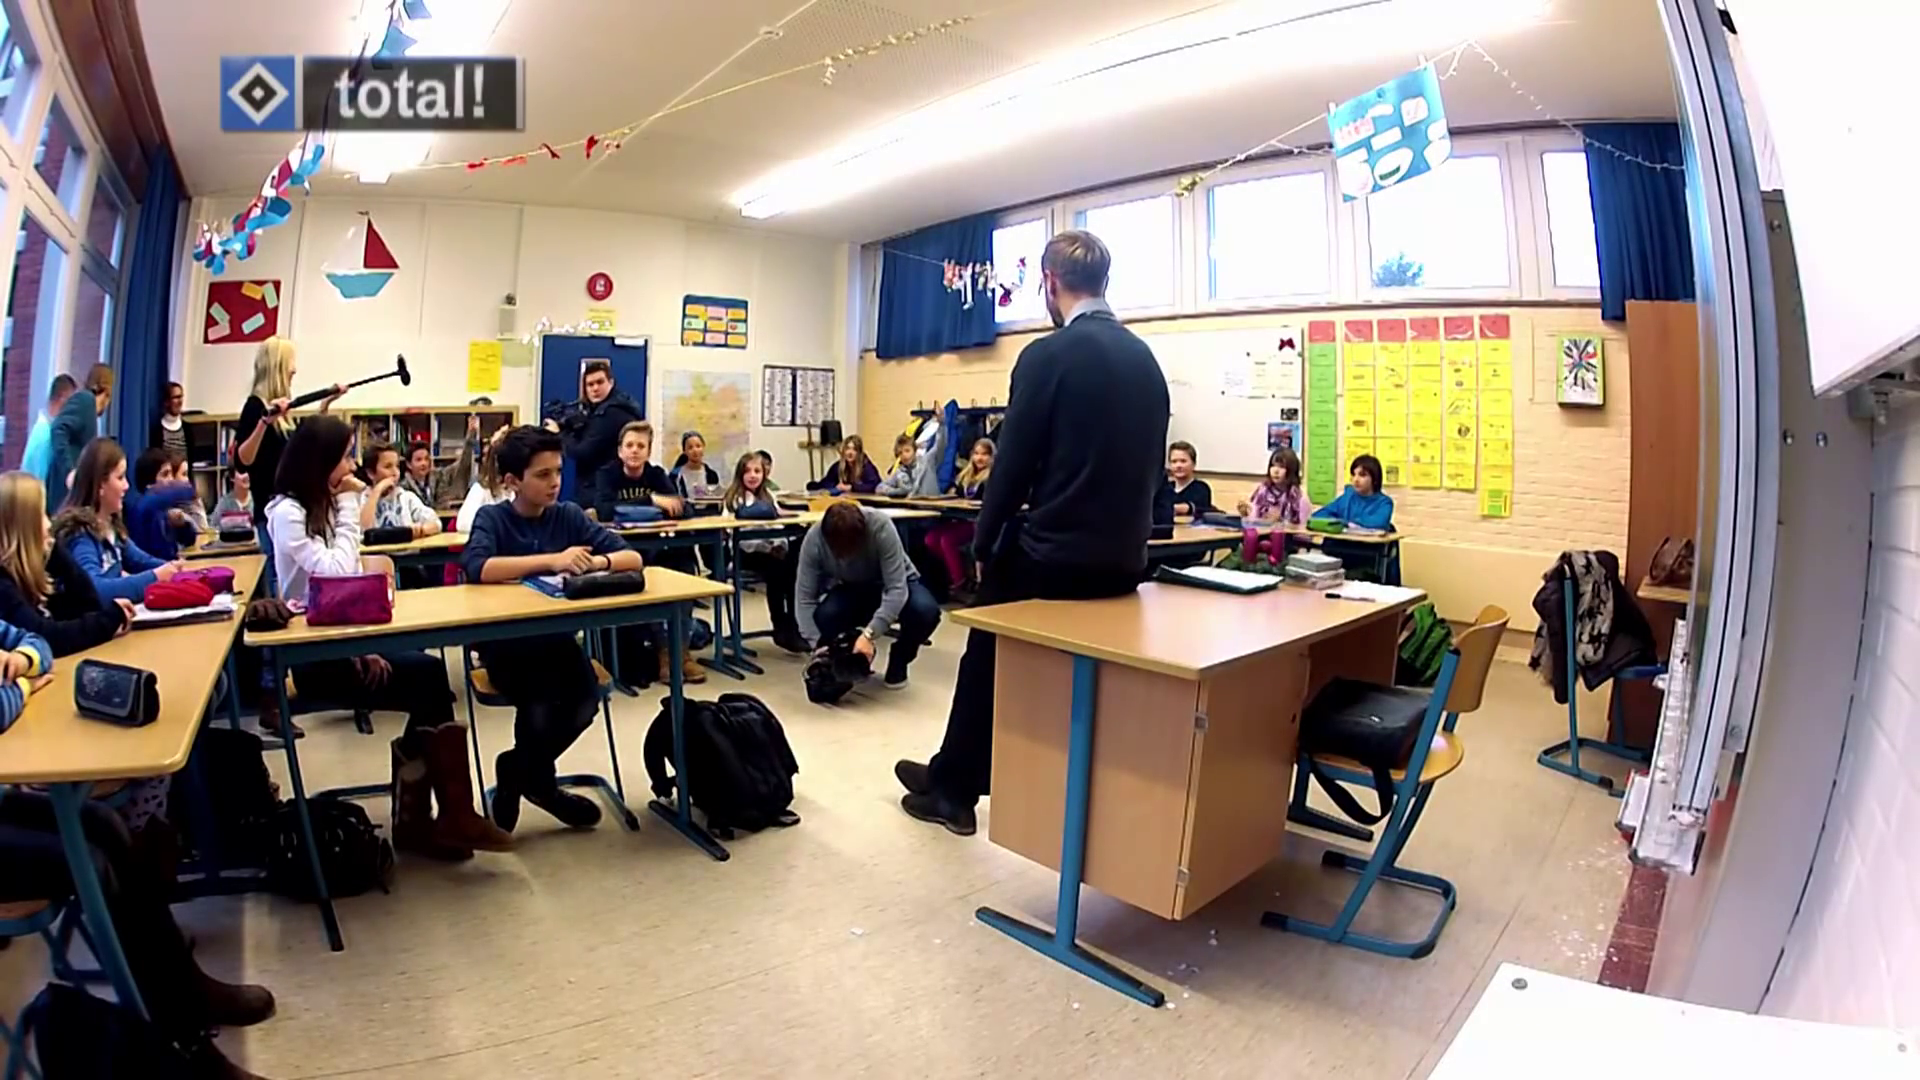
\includegraphics[width=0.7\linewidth]{img/Schulklasse}
	\caption{Eine Screenshot des YouTube-Videos \glqq Maxi Beister als Herr Müller überrascht eine Schulklasse\grqq \cite{Schulklasse_Video}}
	\label{fig:schulklasse}
\end{figure}
